\chapter{Linguagens, Métodos e \textit{Softwares}}
% ---
Nas seções a seguir serão apresentados as linguagens de programação, os métodos e os \textit{softwares} utilizados na construção do sistema proposto.
% ---
\section{Linguagens}
As lingaugens de programação que foram utilizadas para a implementação do sistema estão presentes nesta seção.
\subsection{Python}

Python é uma linguagem de programação interpretada, de alto nível e de uso geral. Criado por Guido van Rossum e lançado pela primeira vez em 1991, a filosofia de design do Python enfatiza a legibilidade do código com seu uso notável de espaço em branco significativo. Suas construções de linguagem e abordagem orientada a objetos têm como objetivo ajudar os programadores a escrever código claro e lógico para projetos de pequena e grande escala.

O Python suporta vários paradigmas de programação, incluindo programação estruturada (principalmente processual), orientada a objetos e funcional. O Python é frequentemente descrito como uma linguagem "baterias incluídas" devido à sua abrangente biblioteca padrão.

Os intérpretes de Python estão disponíveis para muitos sistemas operacionais. Uma organização sem fins lucrativos, a Python Software Foundation, gerencia e direciona recursos para o desenvolvimento de Python. \cite{van2007python}

\subsection{Node.JS}


O Node.JS, também conhecido como Node, é uma estrutura EDA de código aberto para o desenvolvimento de aplicativos JavaScript no servidor. É baseado no \textit{runtime} do Google, chamado de motor V8. O V8 e o Node são implementados em C e C++, focados no desempenho e baixo consumo de memória. Embora o V8 suporte principalmente o uso de JavaScript no navegador, o Node foca no suporte de processos de servidores \cite{Tilkov2010}.

O EDA é uma maneira de realizarmos a comunicação entre sistemas que consiste, principalmente, em operações assíncronas além de permitir aplicativos mais escalonáveis e gerar menos acoplamento entre os serviços, permitindo uma arquitetura fortemente flexível. 

O Node é um dos ambientes e \textit{frameworks} mais famosos que suportam o desenvolvimento de servidores utilizando o JavaScript \cite{Tilkov2010}.



\section{Métodos}
Os métodos e conceitos que foram utilizados para a implementação do sistema estão presentes nesta seção.

\subsection{\textit{Bounding Box}}

As \textit{Bounding Box}(bbox) (Figura \ref{fig:boundingBox}) são um dos métodos de anotação de imagem mais populares e reconhecíveis usados em \textit{Machine Learning} e em \textit{Deep Learning}.

Elas são caixas retangulares que podem ser determinadas pelas coordenadas dos eixos x1 e y1 no canto superior esquerdo e as coordenadas dos eixos x2 e y2 no canto inferior direito do retângulo. Definiremos as \textit{Bounding Boxes} do cachorro e do gato com base nas informações de coordenadas da imagem real.\cite{allDeep}

\begin{figure}[htbp]
		\centering
		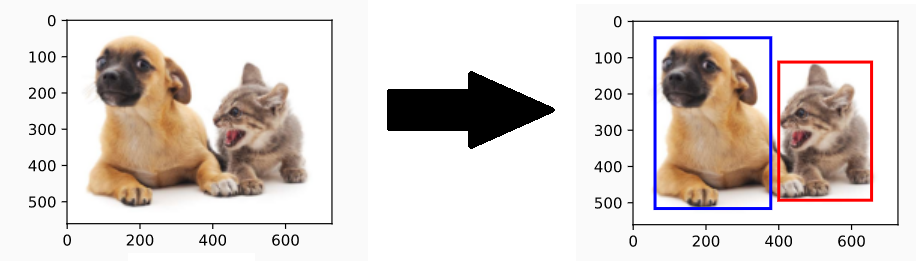
\includegraphics[scale=0.4]{figuras/MachineLearning/catDog.png}
		\caption{Execução de \textit{Bounding Boxes}.}
		\legend{Fonte: \cite{133Ob9905723:online})}
		\label{fig:boundingBox}
\end{figure}

O código \ref{cod:bbox} refere-se à posição das \textit{Bounding Boxes} do cachorro e do gato na imagem, respectivamente.

\begin{lstlisting}[caption=Posições de X e Y nas \textit{Bounding Boxes}, label=cod:bbox]
         dog_bbox, cat_bbox = [60, 45, 378, 516], [400, 112, 655, 493]
\end{lstlisting}


\subsection{\textit{Data Augmentation}}

\textit{Data Augmentation} é o processo de aumentar a quantidade e a diversidade de dados. A partir de imagens originais, gerar mais imagens semelhantes através de vários métodos como, girar 25º, 90º, 45º, embaçar a imagem, entre outros para que possa agrupar em um dataset mais robusto.

Quanto mais dados um algoritmo de ML tiver acesso, mais eficaz ele poderá ser. Mesmo quando os dados são de qualidade inferior, os algoritmos podem ter um desempenho melhor, desde que dados úteis possam ser extraídos pelo modelo do conjunto de dados original. Por exemplo, os modelos de conversão de texto em fala e em texto melhoraram significativamente devido ao lançamento de um corpus de trilhões de palavras pelo Google \cite{halevy2009unreasonable}. Esse resultado ocorre apesar dos dados serem coletados de páginas da Web não filtradas e conter muitos erros. Com esses conjuntos de dados grandes e não estruturados, no entanto, a tarefa passa a ser a de encontrar estrutura dentro de um mar de dados não estruturados. \cite{dataAug}

\subsection{TensorFlow}

O TensorFlow é uma interface para expressar algoritmos de \textit{Machine Learning} e uma implementação para a execução de tais algoritmos. Um cálculo expresso usando o TensorFlow pode ser executado com pouca ou nenhuma alteração em uma ampla variedade de sistemas heterogêneos, desde dispositivos móveis como telefones e tablets até sistemas distribuídos em larga escala de centenas de máquinas e milhares de dispositivos computacionais, como Placas de GPU. 

O sistema é flexível e tem sido usado para conduzir pesquisas e implantar sistemas de aprendizado de máquina na produção em mais de uma dúzia de áreas da ciência da computação e outros campos, incluindo reconhecimento de fala, visão computacional, robótica, recuperação de informações, processamento de idiomas, extração de informações geográficas e descoberta computacional de drogas. \cite{abadi2016tensorflow}

Vários serviços do Google uilizam o TensorFlow em sua produção, o lançaram como um projeto de código aberto e
tornou-se amplamente utilizado para pesquisa de ML.\cite{199317}

\subsection{Scikit-Image}

O Scikit-image, também conhecido como Skimage, é uma biblioteca de processamento de imagens que implementa algoritmos e utilitários para uso em aplicações de pesquisa, educação e indústria. É lançado sob a licença liberal de código aberto Modified BSD, fornece uma API bem documentada na linguagem de programação Python e é desenvolvido por uma equipe internacional ativa de colaboradores.

O objetivo do scikit-image é fornecer uma biblioteca de alta qualidade de ferramentas poderosas e diversas de processamento de imagens, gratuitas e sem restrições. Esses princípios são a base para as práticas de desenvolvimento na comunidade de imagens scikit.\cite{skimage}

\subsection{ImageAI}

ImageAI é uma biblioteca python de código aberto criada para capacitar os desenvolvedores a criar aplicativos e sistemas com recursos independentes de \textit{Deep Learning} e \textit{Computer Vision} usando simples e poucas linhas de código.

A biblioteca ImageAI suporta previsão e treinamento de imagens usando 4 algoritmos diferentes de \textit{Machine Learning} treinados no conjunto de dados ImageNet-1000. O ImageAI também suporta detecção de objetos, detecção de vídeo e rastreamento de objetos usando RetinaNet, YOLOv3 e TinyYOLOv3 treinados no conjunto de dados COCO e PASCAL VOC.\cite{ImageAI}

\subsection{YOLOv3}

A rede neural YOLOv3 evoluiu de YOLO e YOLO-V2 \cite{redmon2018yolov3}. Comparado com a rede Faster R-CNN, em que é a mais eficiente das CNNs quando, a YOLO transforma o problema de detecção em um problema de regressão. Isto não requer uma região da proposta e gera coordenadas e probabilidades de \textit{bounding boxes} de cada classe diretamente por meio de regressão. Isso aumenta consideravelmente a velocidade de detecção em comparação com o Faster R-CNN.\cite{yolov3_apple}

Comparando a rede Faster R-CNN com a  R-CNN, a velocidade do treinamento  é 9 vezes mais rápida e a velocidade do teste é 213 vezes mais rápida. \cite{7960069}

\begin{figure}[htbp]
		\centering
		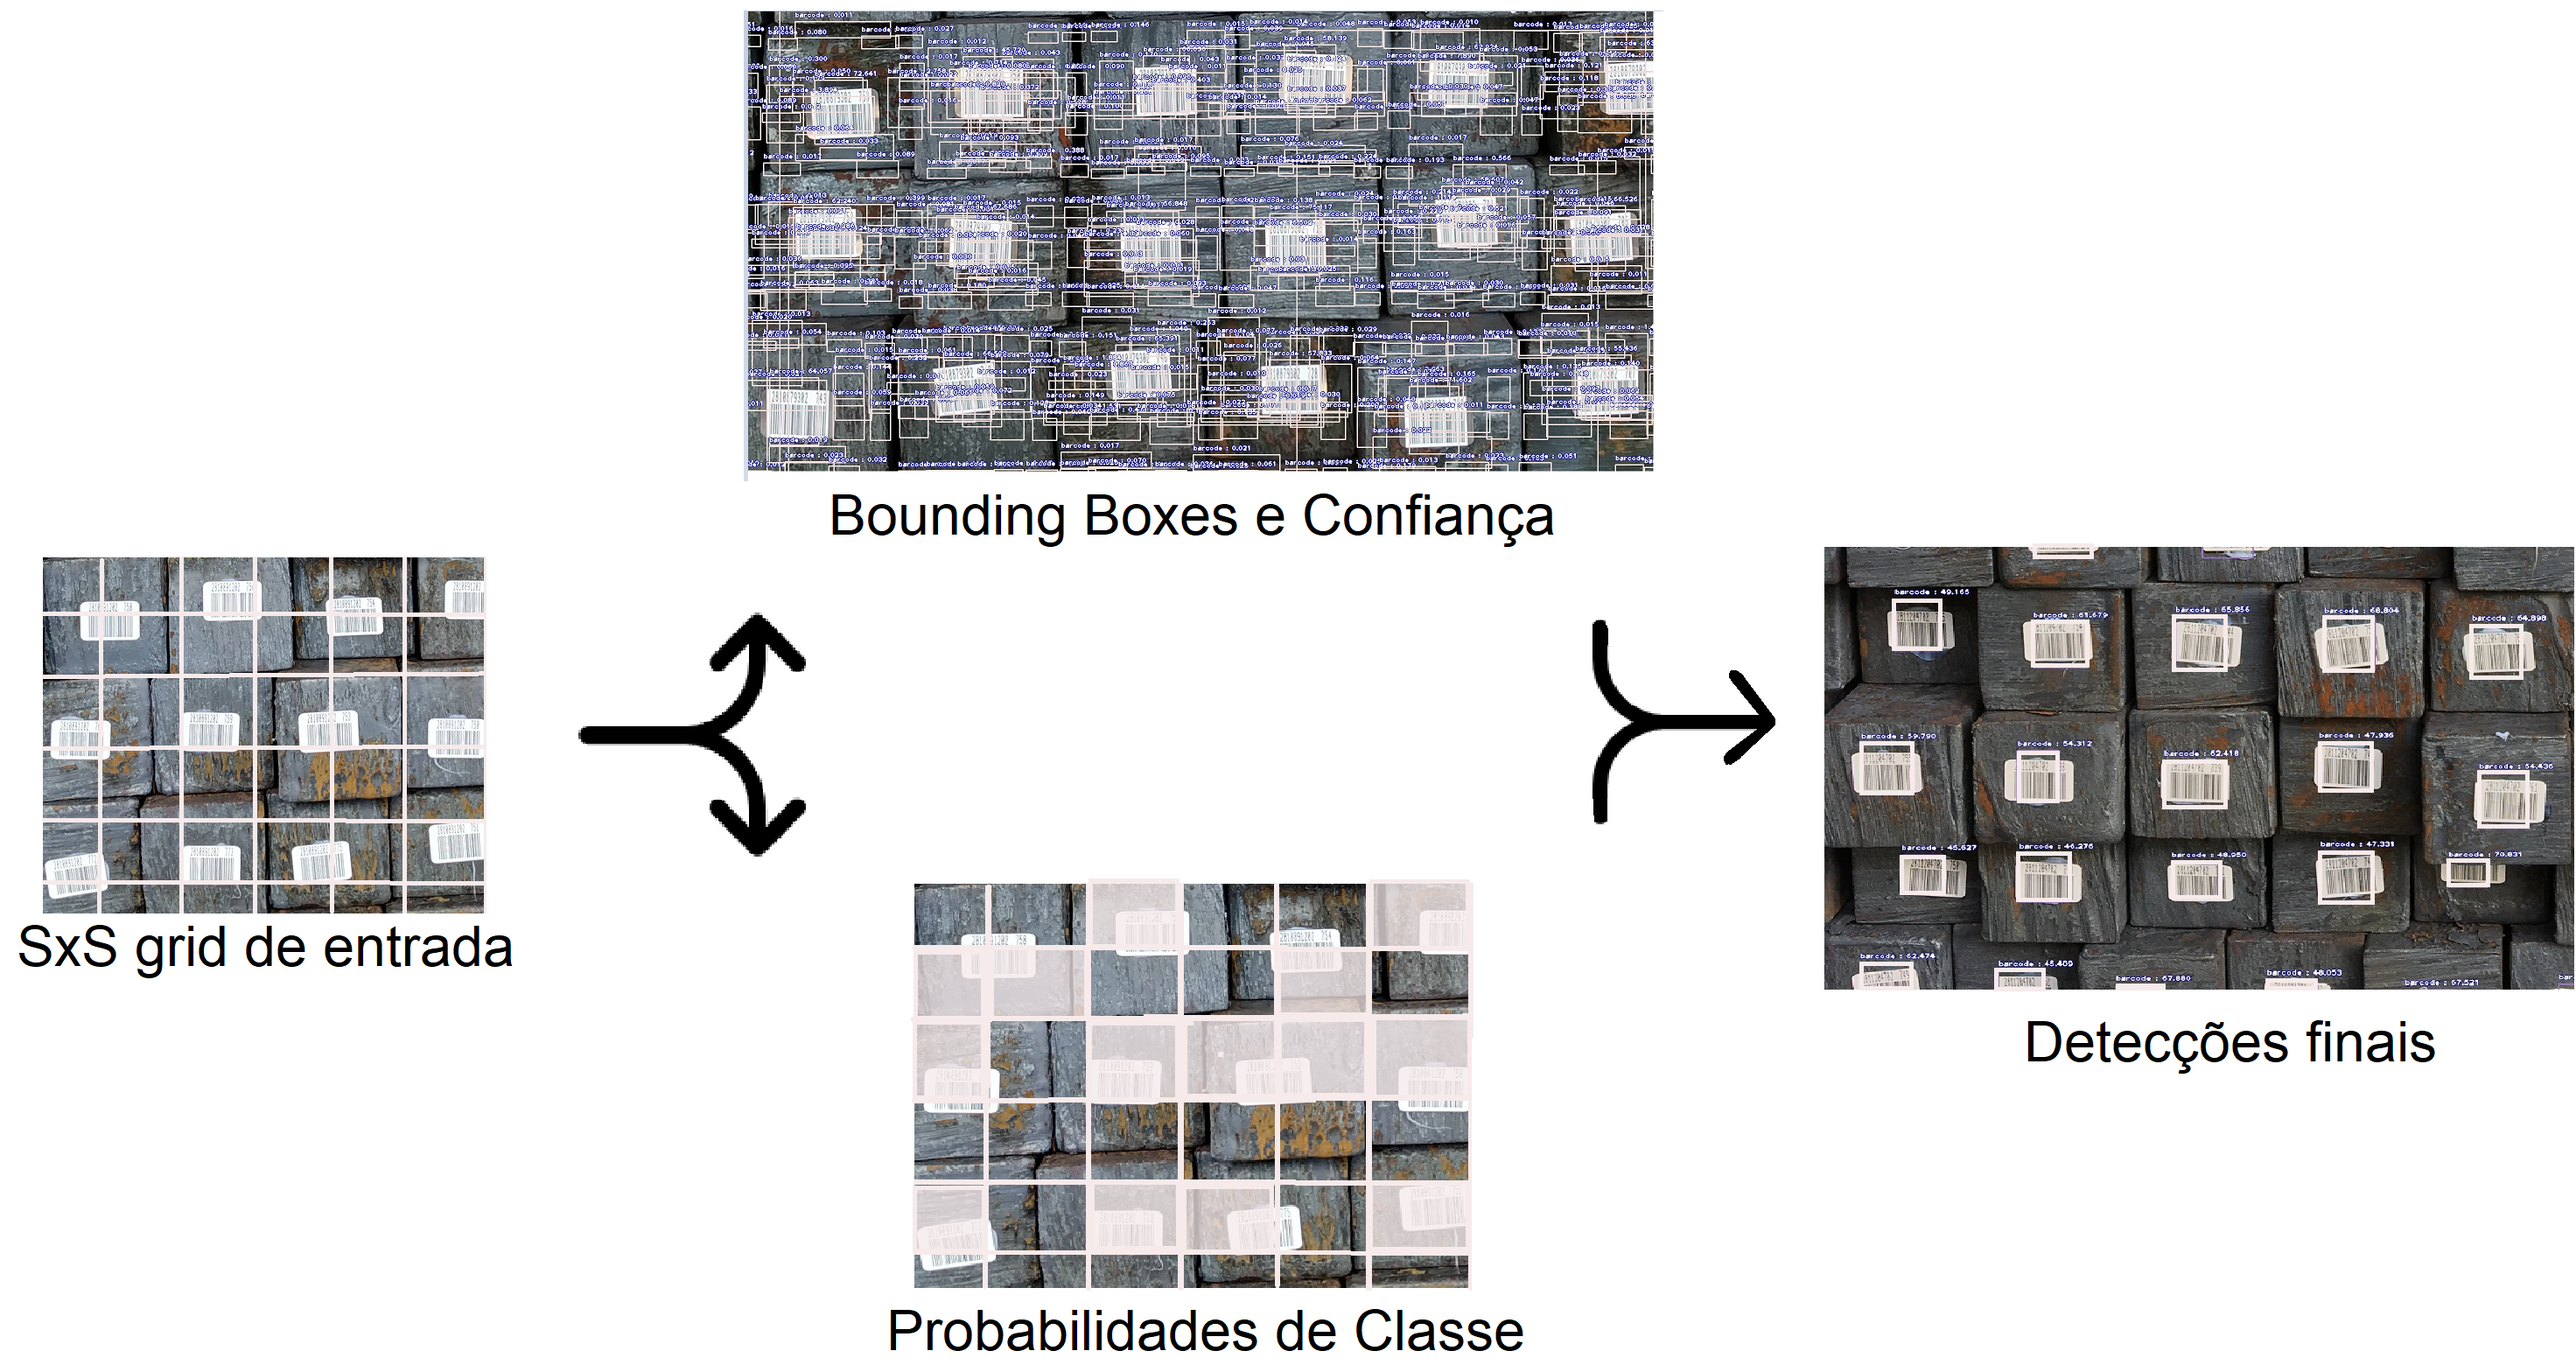
\includegraphics[scale=0.2]{figuras/MachineLearning/yolo.png}
		\caption{YOLO}
		\label{fig:yolo}
\end{figure}

No modelo de detecção YOLO (Figura \ref{fig:yolo}) uma única rede convolucional prediz tanto os \textit{bounding boxes} quanto as probabilidades de pertinencia a classe de cada objeto detectado. Para isso, YOLO funciona da seguinte forma:

\begin{itemize}
    \item Toma-se uma imagem e divide-se-a em um grid SxS de células (S = 6);
    \item Usando o \textit{grid} como referência, gera-se N \textit{bounding boxes};
    \item \textit{Bounding boxes} com probabilidade acima de um limiar são selecionados e usados para localizar o objeto dentro da imagem.
    \item
\end{itemize}

Cada célula do  \textit{grid} é usada para predizer B  \textit{bounding boxes} (bbox) e C probabilidades de classe. O conceito de interseção sobre união (IoU) tem um papel importante e a confiança de uma predição em YOLO é dada por:

\begin{lstlisting}[caption=Posições de X e Y nas \textit{Bounding Boxes}, label=cod:confianca]
        \textit{Confiança = \[ p_r(Object) X IoU_{pred}^truth, p_r(Object) \in {0,1}\]}
\end{lstlisting}

Em que, quando o \textit{target} estiver na \textit{grid}, \[p_r(Object)\] = 1 e 0 caso contrário. A verdade IoUpred é usada para denotar a coincidência entre a referência e a caixa delimitadora prevista. A confiança reflete se a grade contém objetos e a precisão da caixa delimitadora prevista quando ela contém objetos. Quando várias caixas delimitadoras detectam o mesmo destino, o YOLO usa o método de não supressão máxima (NMS) para selecionar a melhor caixa delimitadora.


\section{Softwares}
Os softwares que foram utilizados para a implementação do sistema estão presentes nesta seção.
% ---
\subsection{Google Colaboratory}
O Google Colaboratory, mais conhecido como "Google Colab" ou simplesmente "Colab", é um projeto de pesquisa para criar protótipos de modelos de \textit{Machine Learning} em poderosas opções de \textit{hardware}, como GPUs e TPUs. Ele fornece um ambiente de notebook Jupyter sem servidor para desenvolvimento interativo. O Google Colab é gratuito para usar como outros produtos do G Suite — que anteriormente era conhecido como Google Apps — no qual é um serviço oferecido pelo Google que fornece diversas ferramentas da própria empresa. Elas podem ser totalmente personalizadas com as informações do negócio, incluindo um domínio próprio.

Além de ser fácil de usar, o Colab é bastante flexível em sua configuração e faz muito do trabalho pesado para você. \cite{colabdetail}

\begin{itemize}
    \item Suporte para Python 2.7 e Python 3.6;
    \item Aceleração de GPU grátis;
    \item Bibliotecas pré-instaladas: Todas as principais bibliotecas Python, como o TensorFlow, o Scikit-learn, o Matplotlib, entre muitas outras, estão pré-instaladas e prontas para serem importadas;
    \item Construído com base no Jupyter Notebook;
    \item Recurso de colaboração (funciona com uma equipe igual ao Google Docs): o Google Colab permite que os desenvolvedores usem e compartilhem o Jupyter notebook entre si sem precisar baixar, instalar ou executar qualquer coisa que não seja um navegador;
    \item Suporta comandos \textit{bash};
    \item Os notebooks do Google Colab são armazenados no drive.
\end{itemize}

\begin{figure}[htbp]
		\centering
		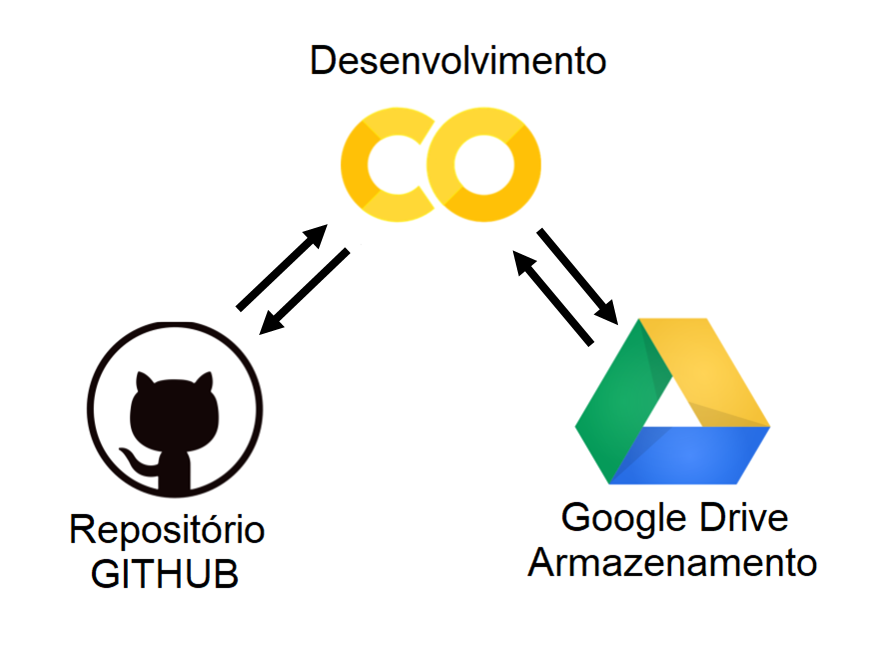
\includegraphics[scale=0.4]{figuras/MachineLearning/colabGithub.png}
		\caption{Utilização do Colab, Drive e Github}
		\label{fig:colabGithub}
\end{figure}

O Colab se integra facilmente ao Google Drive, o que o torna uma opção natural para espaço de armazenamento, em que se armazena os dados e os modelos. Ao mesmo tempo, o Github é mais adequado para hospedagem de código e uso de diversas  bibliotecas gratuitas disponíveis pela comunidade. 

\subsection{LabelImg}

O labelImg (Figura \ref{fig:labelimg}) é uma ferramenta open source de anotação de imagem gráfica escrita em Python. As anotações são salvas em arquivos XML no formato PASCAL VOC (Figura \ref{fig:labelXml}), o formato usado pelo ImageNet. Além disso, também suporta o formato YOLO no qual utilizaremos em nosso projeto. \cite{labelimg}

O software em questão permite que você circule as \textit{bounding boxes} englobando o objeto de interesse nas imagens e criando automaticamente um arquivo XML com todas as especificações necessárias.

Utiliza-se a ferramenta para formar o \textit{dataset}, que é um dos fundamentos da \textit{deep learning}. Para muitos pesquisadores obter dados suficientes para realizar o experimento por si só é um grande problema, por isso precisamos de muitos \textit{datasets open source} para que todo mundo possa usar. Alguns \textit{datasets} comumente usados na visão computacional são os seguintes.

\begin{figure}[htbp]
	\centering
	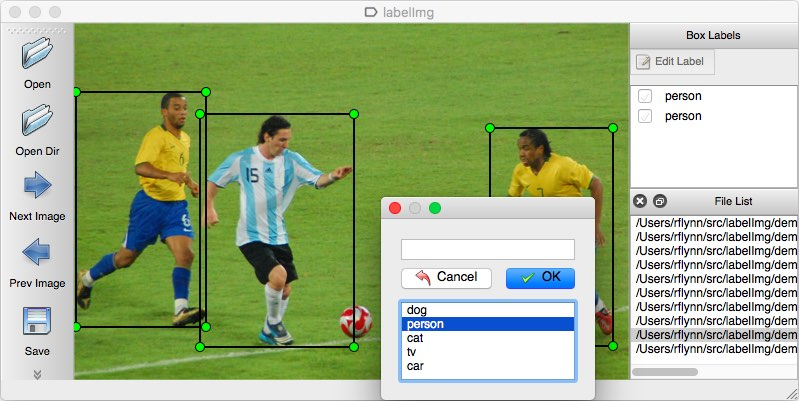
\includegraphics[width=0.9\linewidth]{figuras/MachineLearning/labelimg.jpg}
	\caption{Procedimento de anotações das \textit{bounding boxes}}
	\legend{Fonte: \citeauthor{labelimg} (\citeyear{labelimg})}
	\label{fig:labelimg}
\end{figure}

\begin{figure}[htbp]
	\centering
	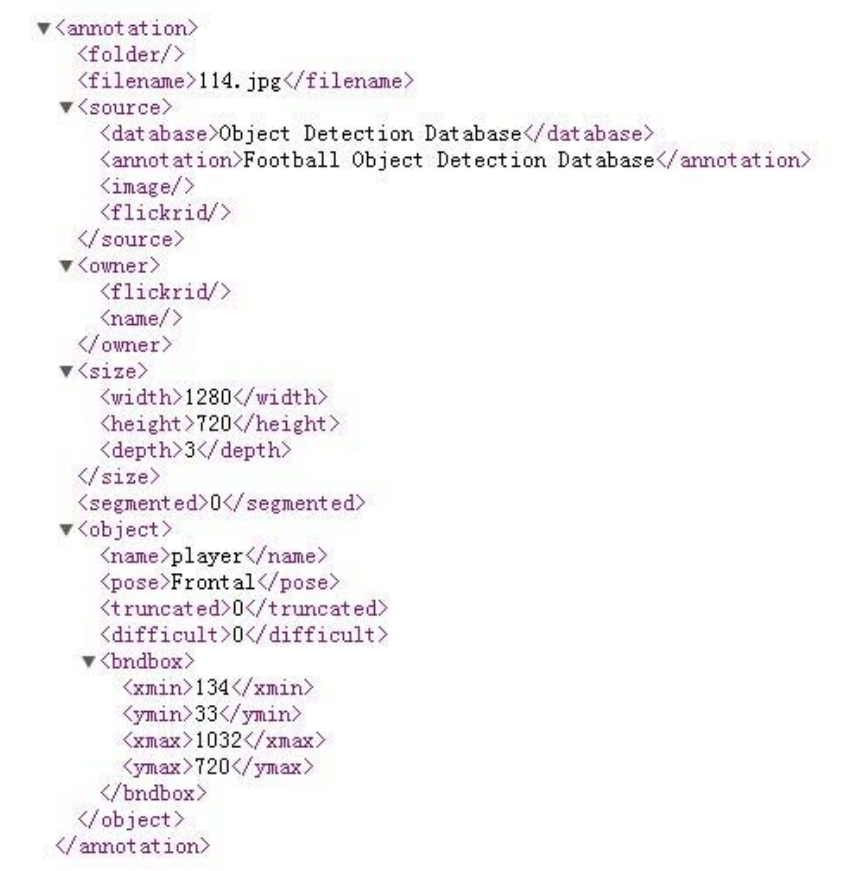
\includegraphics[width=0.8\linewidth]{figuras/MachineLearning/labelXml.png}
	\caption{Arquivo XML gerado pelo LabelImg}
	\legend{Fonte: \citeauthor{zhou2017application} (\citeyear{zhou2017application})}
	\label{fig:labelXml}
\end{figure}

O ImageNet dataset \cite{deng2009imagenet} possui mais de 14 milhões de imagens, cobrindo mais de 20.000 categorias. Existem mais de um milhão de imagens com anotações explícitas de classe e anotações de locais de objetos na imagem. O conjunto de dados Imagenet é um dos conjuntos de dados mais usados no campo da aprendizagem profunda. A maior parte do trabalho de pesquisa, como classificação, localização e detecção de imagens, é baseada nesse conjunto de dados. O conjunto de dados Imagenet é detalhado e é muito fácil de usar. É amplamente utilizado no campo da pesquisa em visão computacional e se tornou o conjunto de dados 'padrão' do aprendizado profundo atual do domínio da imagem para testar o desempenho do algoritmo. \cite{zhou2017application}

O PASCAL VOC (análise de padrões, modelagem estatística e classes de objetos visuais de aprendizado computacional) \cite{everingham2007pascal} fornece conjuntos de dados de imagem padronizados para reconhecimento de classe de objetos e fornece um conjunto comum de ferramentas para acessar os conjuntos de dados e anotações. O conjunto de dados PASCAL VOC inclui 20 classes e tem um desafio baseado nesse conjunto de dados. O PASCAL VOC Challenge \cite{everingham2010pascal} não está mais disponível após 2012, mas seu conjunto de dados é de boa qualidade e bem marcado e permite a avaliação e comparação de diferentes métodos. E como a quantidade de dados do conjunto de dados PASCAL VOC é pequena, comparada ao conjunto de dados imagenet, muito adequada para os pesquisadores testarem programas de rede. Nosso conjunto de dados também é criado com base no padrão de conjunto de dados PASCAL VOC.\cite{zhou2017application}





\section{Sensores e atuadores}

Nesta seção serão apresentados os sensores e atuadores a terem seus sinais utilizados no projeto. 

\subsection{Sensor de fluxo YF-S201} \label{sec:sensor}

O sensor YF-S201 (Figura \ref{fig:sensor}) é um sensor do tipo turbina que mede a quantidade de líquido que passa pela tubulação, girando aletas que
geram pulsos de onda quadrada através de um sensor de efeito Hall \cite{roque2018sistema}. O
sensor usa esse efeito para enviar um sinal PWM (\textit{Pulse Width Modulation}) e, através da contagem deste sinal é possível mensurar a quantidade de água que passa pela turbina no interior do sensor. \cite{ms2017automaccao}

\begin{figure}[htbp]
		\centering
		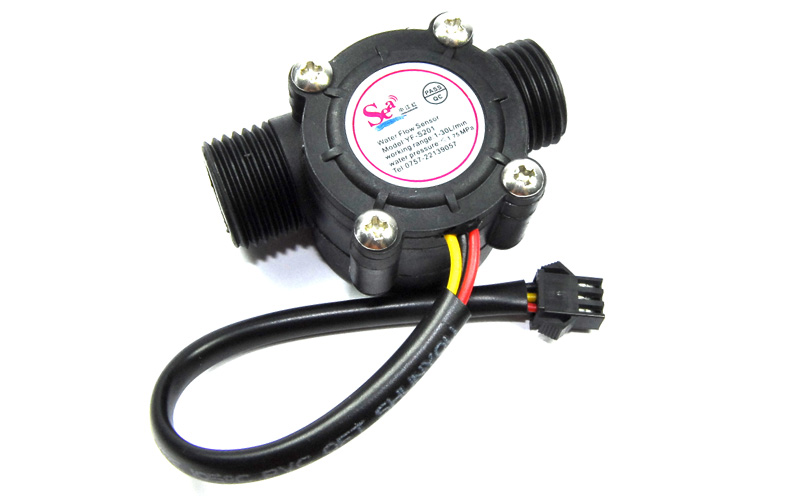
\includegraphics[scale=0.3]{figuras/yf-s201.jpg}
		\caption{Sensor de fluxo de água YF-S201.}
		\label{fig:sensor}
\end{figure}

\newpage

\subsection{Teclado matricial de membrana} \label{sec:teclado}

Teclados permitem que usuários insiram informações em diversos tipos de sistemas, como computadores, calculadoras, controles remotos entre outros \cite{teclado-matricial-1}. O Teclado Matricial de Membrana 4X4 (Figura \ref{fig:teclado}) foi desenvolvido com a finalidade de facilitar a entrada de dados em projetos com plataformas microcontrolada \cite{teclado-matricial}. Este teclado possui 16 teclas, sendo 10 teclas são numéricas, 4 literais e 2 caracteres especiais.

\begin{figure}[htbp]
	\centering
	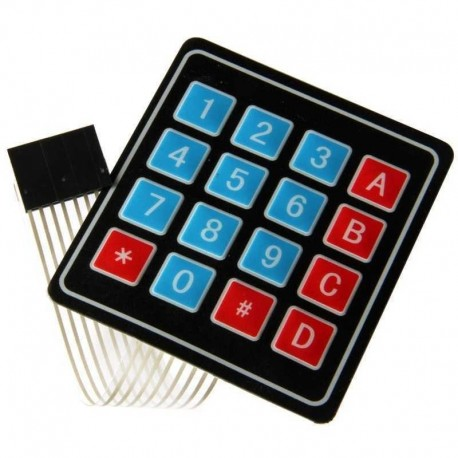
\includegraphics[scale=0.2]{figuras/teclado-matricial.jpg}
	\caption{Teclado Matricial de Membrana.}
	\legend{Fonte: \citeauthor{teclado-matricial-1} (\citeyear{teclado-matricial-1})}
	\label{fig:teclado}
\end{figure}

As teclas estão dispostas em 4 linhas por 4 colunas e o teclado possui um conector de 8 pinos para ligação. Quando um botão do teclado é pressionado, ele conecta a linha com a coluna na qual está ligado, gerando um sinal nos pinos referente àquela linha/coluna. Este sinal permite a identificação da tecla apertada pelo sistema. O circuito do teclado está exemplificado na Figura \ref{fig:teclado-conexoes}.

\begin{figure}[htbp]
	\centering
	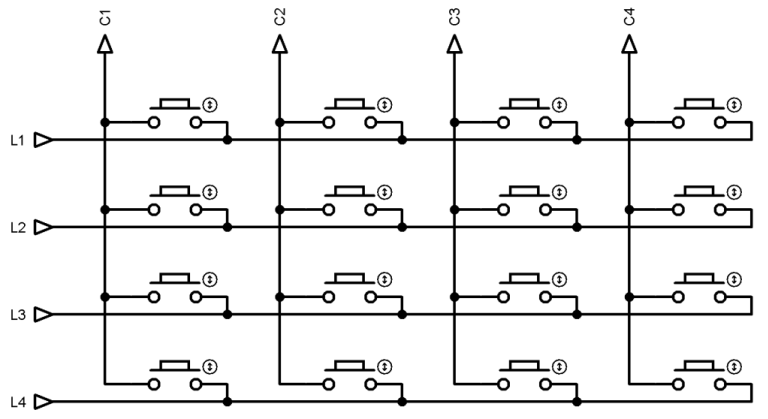
\includegraphics[scale=0.4]{figuras/matrix-1024x558.png}
	\caption{Circuito do teclado.}
	\legend{Fonte: \citeauthor{teclado-matricial} (\citeyear{teclado-matricial})}
	\label{fig:teclado-conexoes}
\end{figure}

A Tabela \ref{table:pinosteclado} possui as informações da distribuição dos pinos em tabelas e colunas, exemplificada na Figura \ref{fig:teclado-pins}.

\begin{table}[h!]
	\begin{center}
		\begin{tabular}{ |c|c| }
			\hline
			\rowcolor{lightgray} Pino & Localização \\
			 \hline 
				1 & Linha 1 \\
			 \hline 
				2 & Linha 2 \\
			 \hline 
				3 & Linha 3 \\
			 \hline 
				4 & Linha 4 \\
			 \hline 
				5 & Coluna 1 \\
			 \hline 
				6 & Coluna 2 \\
			 \hline 
				7 & Coluna 3 \\
			 \hline 
				8 & Coluna 4 \\
			\hline
		\end{tabular}
	\caption{Tabela de disposição dos pinos do teclado numérico.}
	\label{table:pinosteclado}
	\end{center}
\end{table}

\begin{figure}[htbp]
	\centering
	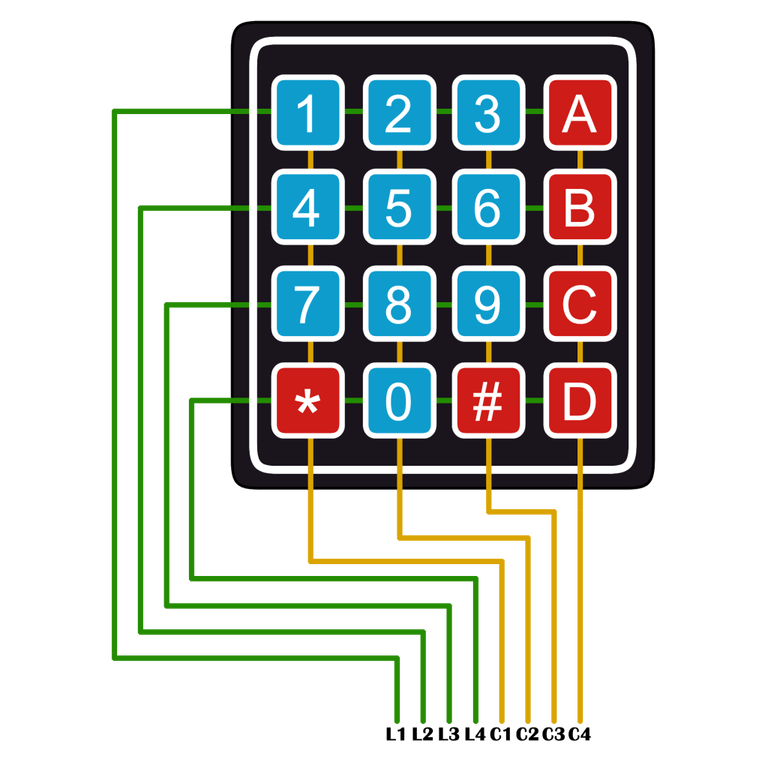
\includegraphics[scale=0.3]{figuras/keypad-1024x1024-pins.png}
	\caption{Pinagem do teclado.}
	\legend{Fonte: \citeauthor{teclado-matricial} (\citeyear{teclado-matricial})}
	\label{fig:teclado-pins}
\end{figure}

\newpage

\subsection{Válvula solenoide} \label{sec:valvula}

Solenóides são dispositivos eletromecânicos baseados no deslocamento causado pela ação de um campo magnético gerado por uma bobina e são muito utilizados na construção de outros dispositivos, como é o caso das válvulas para controle de fluidos. Em particular, as válvulas para baixas vazões (da ordem de mililitros por minuto) e baixas pressões têm sido amplamente aplicadas em equipamentos e montagens para uso em laboratórios clínicos e químicos  \cite{da2002modulo}. Elas são de pequenas dimensões e requerem baixa tensão e corrente de acionamento.

A válvula solenoide pode ser vista na Figura \ref{fig:valvula-solenoide}.

\begin{figure}[htbp]
	\centering
	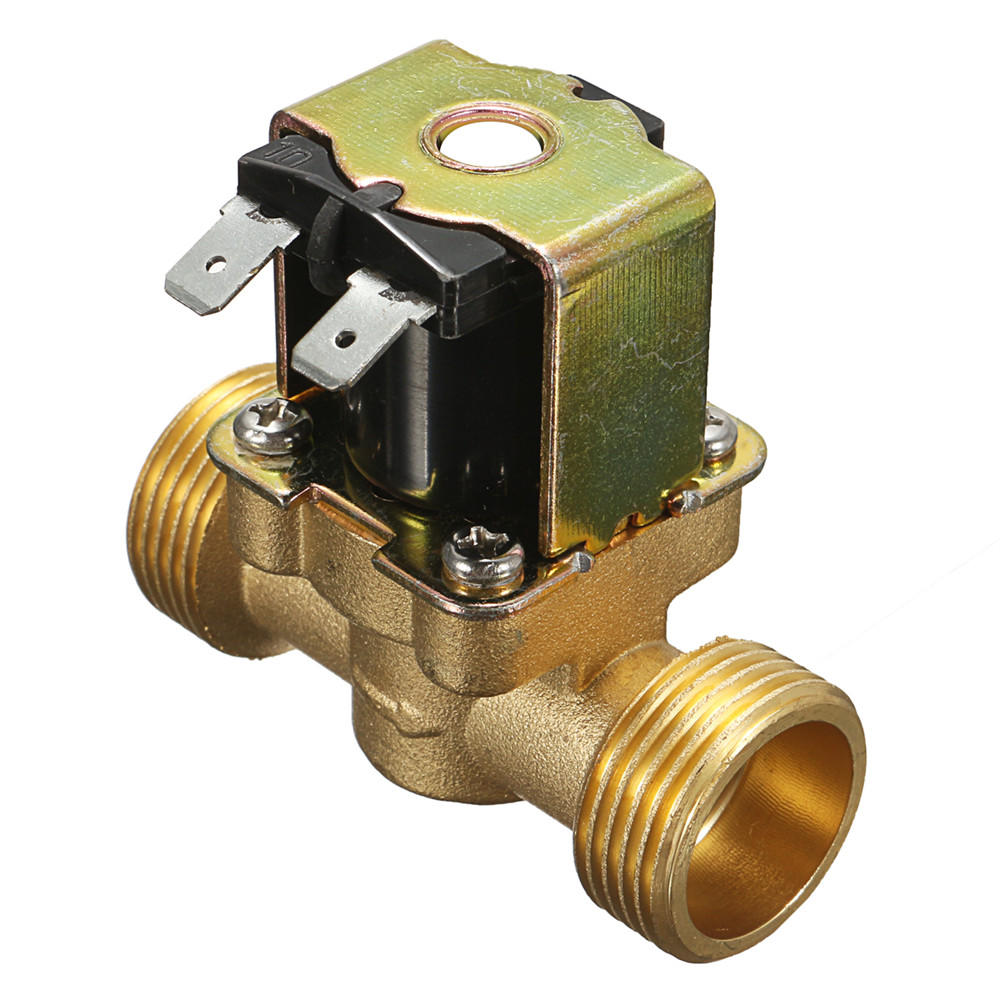
\includegraphics[width=0.3\linewidth]{figuras/valvula-solenoide.jpg}
	\caption{Válvula Solenoide.}
	\label{fig:valvula-solenoide}
\end{figure}

Segundo \citeauthor{da2002modulo} (\citeyear{da2002modulo}), a estratégia para fechamento e abertura dos canais fluídicos depende do fabricante, mas o princípio de acionamento elétrico é comumente o mesmo. Uma tensão é aplicada sobre um solenoide, criando um campo magnético que desloca um núcleo ferromagnético móvel, causando a alteração do estado da válvula. O núcleo
ferromagnético comprime uma mola que é a responsável por retornar o núcleo a sua posição original quando a corrente elétrica é interrompida.

\section{Softwares}

Os softwares que foram utilizados para a implementação do sistema estão presentes nesta seção.

\subsection{HomeAssistant}

O HomeAssistant é um plataforma de automação escrita em Python. Inclui componentes contribuídos por usuários que permite a interface com Web Services e dispositivos como sensores, microcontroladores e assistentes virtuais \cite{Lundrigan2017}. Em seu núcleo, o HomeAssistant é um protocolo de troca de mensagens que facilita a comunicação entre dispositivos e componentes funcionais na rede. Provendo simples abstrações de componentes de automação residencial como sensores, câmeras, \textit{players} de música, etc.

A Figura \ref{fig:homeassistant-dash} apresenta um exemplo de tela inicial do HomeAssistant. Com vários sensores configurados na parte superior, na parte esquerda, encontra-se o menu do HomeAssistant, e na parte central inferior pode-se observar informações sobre o clima e \textit{switches} para acionamento de interruptores e iluminação.

\begin{figure}[htbp]
	\centering
	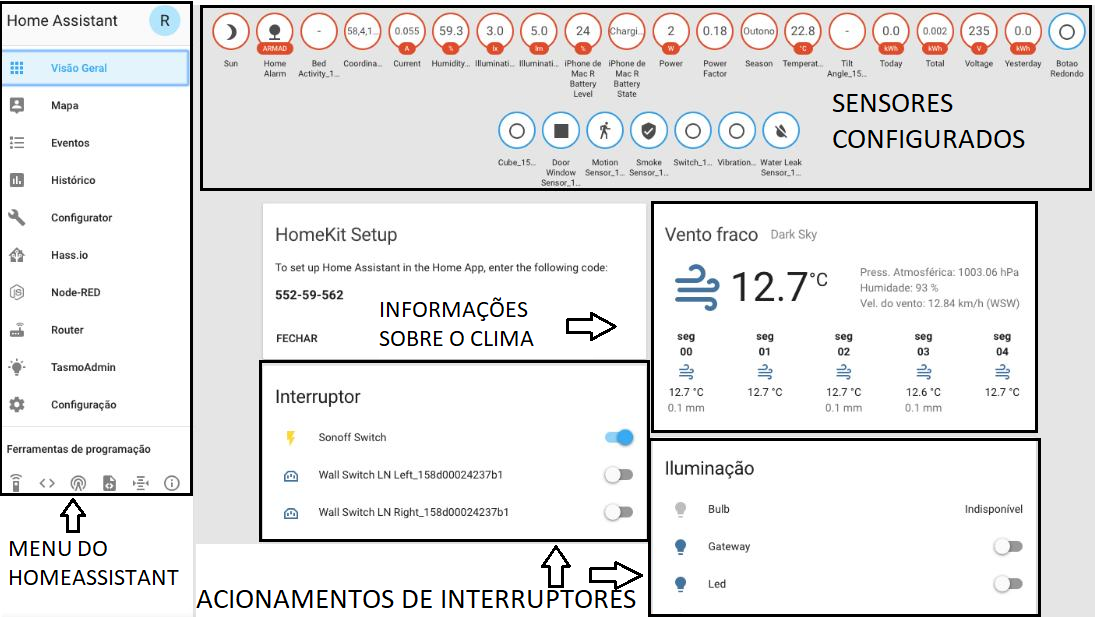
\includegraphics[width=1\linewidth]{figuras/homeassistant-dash.png}
	\caption{Dashboard genérico do HomeAssistant}
	\legend{Fonte: Adaptado de \citeauthor{AlmeidaCosta} (\citeyear{AlmeidaCosta})}
	\label{fig:homeassistant-dash}
\end{figure}

O HomeAssistant tem suporte para diversos tipos de protocolos \textit{wireless}, como BLE, ZigBee, Z-Wave e Wi-Fi. Conta também com um RESTful API e suporta HTTP, MQTT, TCP \textit{sockets} e componentes customizados. Estes componentes customizados permitem aos usuários adicionar funções próprias no HomeAssistant sem a necessidade de mudar o seu código fonte. Isto torna a integração de novos dispositivos e sensores muito mais fácil com o HomeAssistant \cite{Gomes2018}.


%O HomeAssistant conta com uma grande comunidade de desenvolvedores com mais de 1.450 contribuidores e 23.700 estrelas no GitHub\footnote{\url{https://github.com/home-assistant/home-assistant}}, o que significa uma abundância em sua documentação sobre os seus componentes, fóruns e chats para conseguir ajuda de outros usuários, e diversos posts em blogs e vídeos sobre como começar a utilizar o programa.

Tendo em vista a gama de protocolos sem fio disponíveis no HomeAssistant, escolhemos o padrão Wi-Fi pois segundo \citeauthor{Lundrigan2017} (\citeyear{Lundrigan2017}):

\begin{itemize}
	\item O custo dos equipamentos com padrão Wi-Fi é reduzido.
	\item Wi-Fi é o mais difuso dos protocolos wireless.
	\item Sensores Wi-Fi tem integração facilitada com demais equipamentos residenciais.
\end{itemize}

O HomeAssistant pode ser instalado em qualquer sistema operacional devido ao fato de ser muito pequeno e leve. O que o faz ser compatível para o uso no Rasberry Pi como um hub de automação pequeno e barato. É importante lembrar que o HomeAssistant age apenas como uma central de controle que pode informar outros serviços, como o Philips Hue ou o Nest, que são produtos para automação residencial, para realizar alguma função \cite{AlmeidaCosta}. O Home Assistant é gratuito e de fácil configuração.

\subsection{Banco de dados de séries temporais}

Um Banco de Dados de Séries Temporais, do inglês \textit{Temporal Series Database} (TSDB), é um tipo de banco otimizado para dados coletados no tempo. É implementado especificamente para lidar com métricas, eventos ou medidas que variam no tempo. Um TSDB permite o usuário criar, enumerar, alterar, destruir e organizar várias séries temporais de métodos mais eficientes. Atualmente, a maioria das empresas estão gerando um grande volume de dados sobre métricas e eventos que são mapeados no tempo, aumentando a relevância de tal arquitetura \cite{Noor2017}.

Ainda segundo \citeauthor{Noor2017} (\citeyear{Noor2017}), aplicações comuns para os TSDBs são IoT, DevOps e Analise de Dados. Alguns casos de uso incluem monitoramento de sistemas de \textit{software} como máquinas virtuais, monitoramento de sistemas físicos como dispositivos, ambiente, sistemas de automação residencial, dentre outros.

\subsubsection{InfluxDB}

O InfluxDB é o Banco de Dados de Séries Temporais usado neste projeto, sendo o mais apto a guardar os dados de fluxo no tempo. \cite{Lundrigan2017}

É um projeto \textit{open-source} com o opcional de armazenamento pago em nuvem desenvolvido pela empresa InfluxData. É escrito na linguagem de programação Go e baseado em uma linguagem de consulta parecida com o SQL \cite{Noor2017}.

\subsubsection{Grafana}

Grafana é um projeto \textit{open-source} para análise de dados de séries temporais  \cite{Noor2017} que realiza consultas destas séries temporais a partir do InfluxDB exibindo os dados de maneira gráfica \cite{chang2017kubernetes}.

\subsection{Banco de dados relacional}

Um Banco de Dados Relacional é capaz de salvar e referenciar dados para uma consulta posterior. Possui uma coleção de tabelas, todas com identificadores únicos, que compõem a base de
dados. Conceitos como integridade referencial de dados – que garante sincronia de dados entre tabelas – e chaves primárias estão presentes, garantindo que um conjunto de informações possa ser representado de maneira consistente, independente da forma de acesso  \cite{bancosrelacionais}.

\subsubsection{PostgreSQL}

O PostgreSQL é uma implementação de um banco de dados relacional, de código aberto e de custo gratuito \cite{stones2006beginning}. O 
PostgreSQL pode ser usado com diversas linguagens de programação, como por exemplo: Python, Javascript, Java e C++.

O PostgreSQL ganhou diversos prêmios, incluindo o \textit{Linux Journal Editor's Choice Award for Best Database} três vezes e o \textit{2004 Linux New Media Award for Best Database System}.

\subsection{Node.JS}

O Node.JS, também chamado de Node, é um ambiente de servidor que utiliza a linguagem de programação JavaScript. É baseado no \textit{runtime} do Google, chamado de motor V8. O V8 e o Node são implementados em C e C++, focados no desempenho e baixo consumo de memória. Embora o V8 suporte principalmente o uso de JavaScript no navegador, o Node foca no suporte de processos de servidores \cite{Tilkov2010}.

O Node.JS utiliza um paradigma baseado em eventos e não-bloqueador de I/O, o que o torna leve e eficiente. É perfeito para aplicações de tempo real que lidam com dados intensos em dispositivos de baixo poder de processamento \cite{Sapes2016}.

O Node é um dos ambientes e \textit{frameworks} mais famosos que suportam o desenvolvimento de servidores utilizando o JavaScript. A comunidade criou um grande ecossistema de bibliotecas e vasta documentação de suporte ao Node \cite{Tilkov2010}.

\subsection{Arquitetura de microsserviços}

Seguindo a definição de \citeauthor{ms1} (\citeyear{ms1}), a arquitetura de microsserviços trata do desenvolvimento de uma aplicação que baseia na existência de diversos pequenos serviços independentes. Cada um dos serviços deve rodar em seu próprio processo independente. Estes serviços podem comunicar entre si utilizando mecanismos leves de comunicação (geralmente em torno no HTTP). Os serviços devem ser absolutamente independentes.

Um exemplo da arquitetura de microsserviços está na Figura \ref{fig:arquitetura-microsservicos}.

\begin{figure}[htbp]
	\centering
	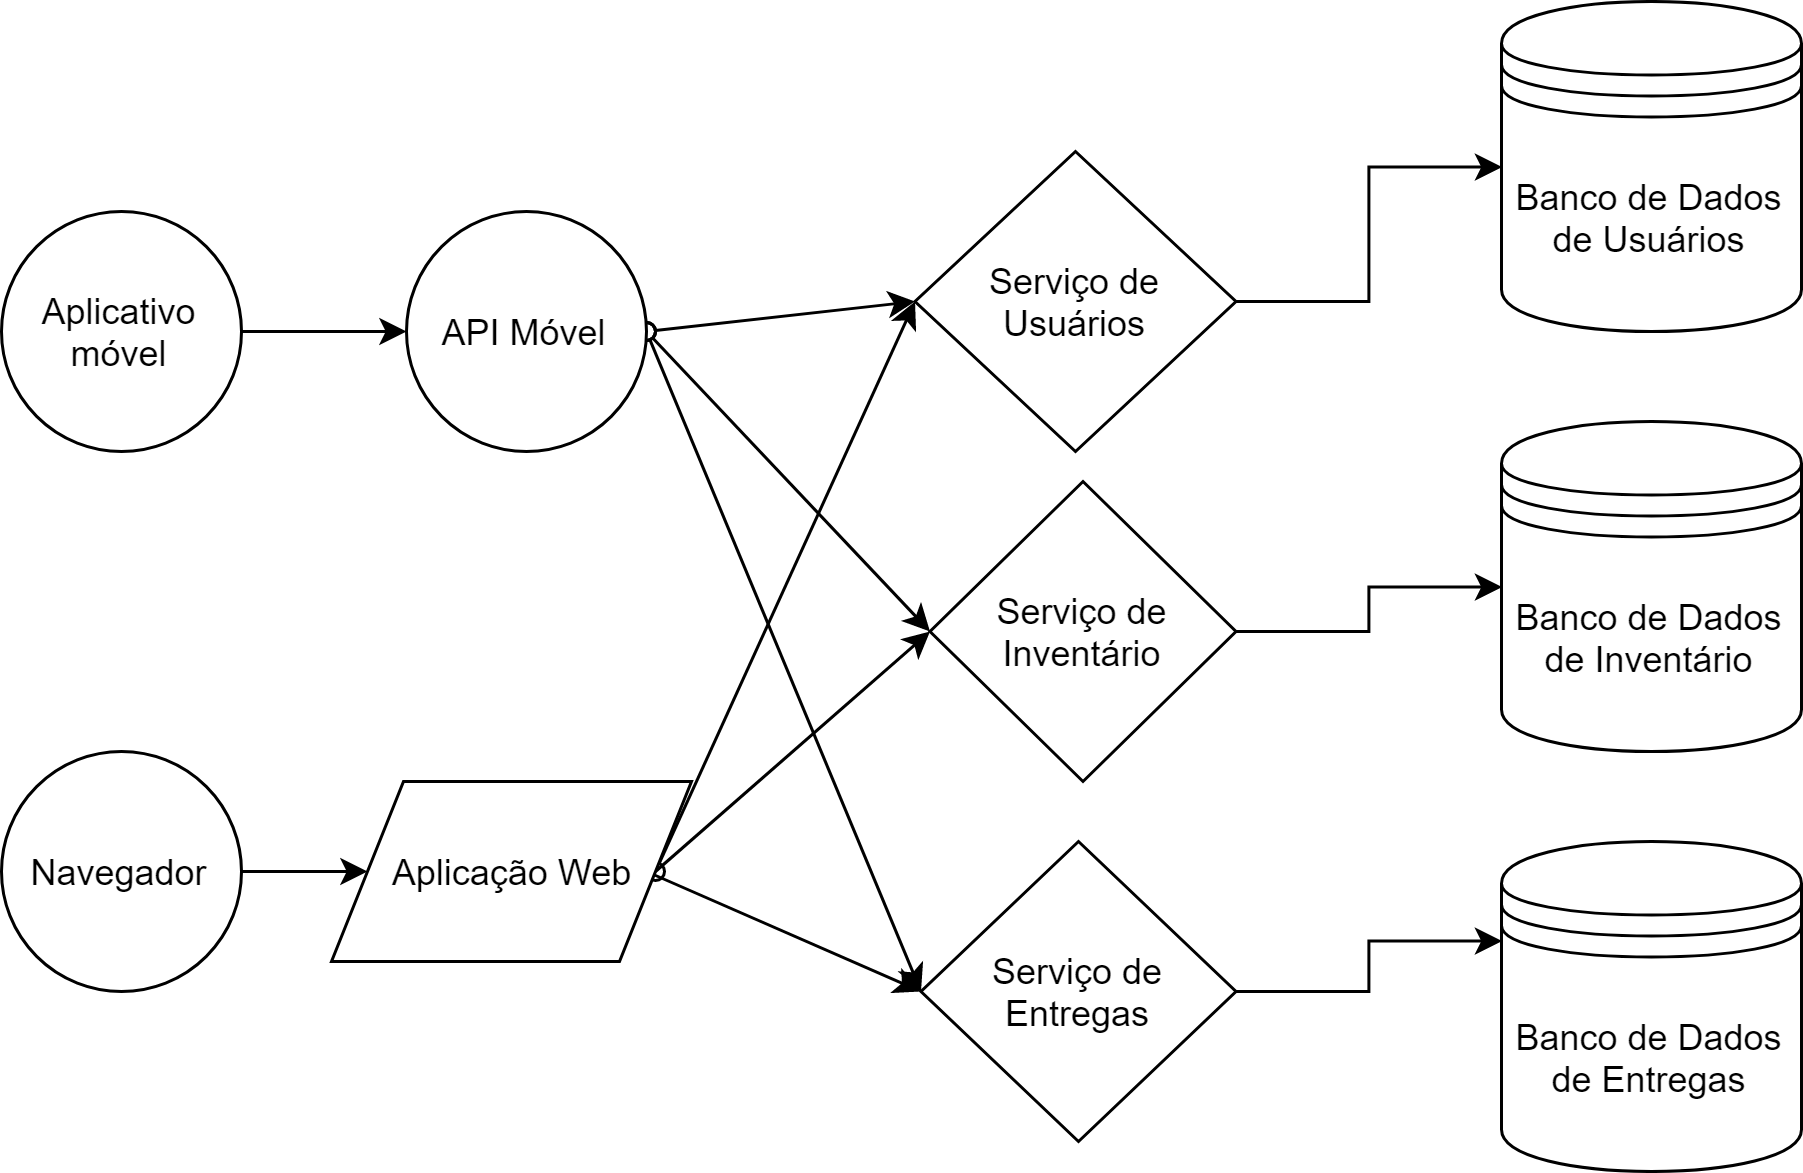
\includegraphics[width=1\linewidth]{figuras/microservices.png}
	\caption{Exemplo arquitetura de microsserviços.}
	\label{fig:arquitetura-microsservicos}
\end{figure}

Microsserviços são os resultados da decomposição funcional de uma aplicação. São caracterizados pela definição de sua interface e função no sistema. Como cada serviço deve ser independente, uma alteração na sua implementação não deve afetar o funcionamento dos demais. \cite{Pahl}

\subsection{Protocolo de comunicação MQTT}

MQTT significa \textit{Message Queuing Telemetry Transport}, traduzido para o português como Transporte de Telemetria de Enfileiramento de Mensagens. É um protocolo de transporte leve que otimiza o uso da a largura de banda de rede\footnote{\url{http://public.dhe. ibm.com/software/dw/webservices/ws-mqtt/mqtt-v3r1.html}}. O MQTT trabalha sobre o protocolo TCP e garante a entrega de mensagens de um nó para um servidor. Sendo um protocolo orientado por troca de mensagens, MQTT é ideal para aplicações IoT, que comumente tem recursos e capacidades limitados.

É um protocolo inicialmente desenvolvido pela IBM\footnote{\url{http://www.hivemq.com/blog/mqtt-essentials-part-1-introducing-mqtt}} em 1999, sendo recentemente reconhecido como padrão pela OASIS (Organizarion for the Advancement of Structured Information Standards)\footnote{\url{https://www.oasis-open.org/news/announcements/ mqtt-version-3-1-1-becomes-an-oasis-standard}}.

\citeauthor{Kodali2017} (\citeyear{Kodali2017}) definiu o MQTT como um protocolo baseado em \textit {publisher/subscriber}. Qualquer conexão MQTT envolve dois tipos de agentes, os clientes e um \textit {broker}, ou servidor. Qualquer dispositivo ou programa que é conectado pela rede e troca mensagens através do MQTT é chamado de cliente. Um cliente pode ser tanto um \textit {publisher} e/ou um \textit {subscriber}. Um \textit {publisher} publica mensagens e um \textit {subscriber} requisita o recebimento de mensagens. Um MQTT \textit {server} é um programa que interconecta os clientes. Ele aceita e transmite as mensagens através de múltiplos clientes conectados à ele.

\begin{figure}[htbp]
	\centering
	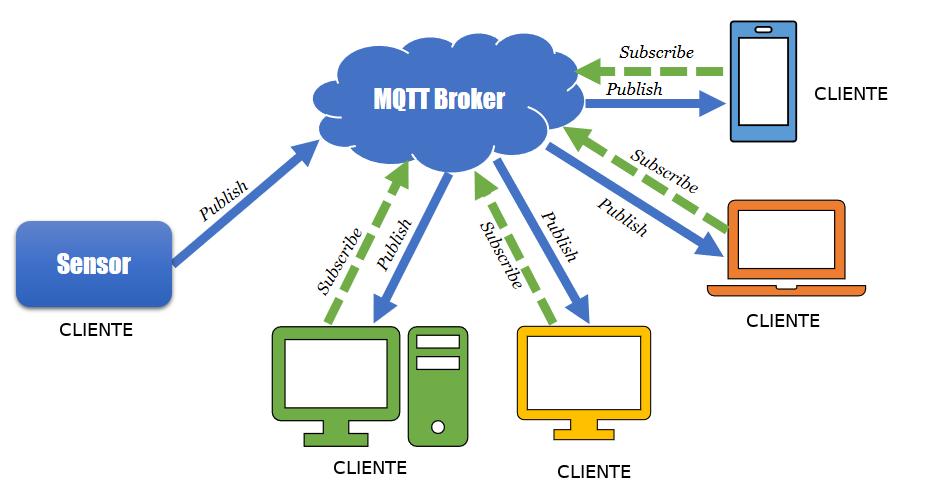
\includegraphics[width=1\linewidth]{figuras/mqtt-architecture.png}
	\caption{Exemplo da arquitetura do MQTT.}
	\legend{Fonte: \citeauthor{embeddedmqtt} (\citeyear{embeddedmqtt})}
	\label{fig:arquitetura-mqtt}
\end{figure}

\newpage

Dispositivos como sensores e celulares podem ser vistos como clientes do ponto de vista da arquitetura MQTT. Quando um cliente tem alguma informação para transmitir, ele publica o dado para o \textit {broker}.

A Figura \ref{fig:arquitetura-mqtt} apresenta um exemplo de arquitetura MQTT comum. O \textit {broker} MQTT, ou servidor MQTT é responsável por coletar e organizar os dados. As mensagens publicadas por clientes MQTT são transmitidas para outros clientes MQTT que se inscreverem ao tópico. O MQTT é desenhado para simplificar a implementação no cliente por concentrar todas as complexidades no \textit {broker}. Os \textit {publishers} e \textit {subscribers} são isolados, o que significa que eles não precisam conhecer a existência do outro.

\subsubsection{MQTT Mosquitto}

O Mosquitto é um \textit{broker} MQTT de código aberto \cite{Kodali2017} que entrega uma implementação de servidor e cliente MQTT. Utiliza o modelo \textit{publisher/subscriber}, tem uma baixa utilização de rede e pode ser implementado em dispositivos de baixo custo como microcontroladores. \cite{Light}

Segundo \citeauthor{Light} (\citeyear{Light}), Mosquitto é recomendado para o uso sempre em que se necessita de mensagens leves, particularmente em dispositivos com recursos limitados.

O Projeto Mosquitto é um membro da Eclipse Foundation. Existem três partes no projeto:

\begin{itemize}
	\item O servidor principal Mosquitto.
	\item Os clientes mosquitto \textit{pub} e mosquitto \textit{sub}, que contém ferramentas para se comunicar com o servidor MQTT.
	\item Uma biblioteca cliente MQTT, escrita em C.
\end{itemize}

%\subsection{Docker}
%
%Docker é um projeto \textit{open source} que foi inicialmente lançado em 2013, atraiu grande atenção na industria de TI. É uma plataforma de conteinerização que possibilita usuários a construir sua aplicação dentro de um conteiner e transferir conteiners através de máquinas com diferentes sistemas operacionais de um jeito simples. \cite{chang2017kubernetes}
%
%Existem três componentes principais do Docker:
%
%\begin{itemize}
%	\item \textit{Docker images}: são \textit{templates} de leitura que servem como base para a criação de conteiners.;
%	\item \textit{Docker registries}: é o local onde estão uma grande coleção de \textit{Docker images}.;
%	\item \textit{Docker containers}: são as instâncias virtuais em que as aplicações estão rodando. Cada conteiner contem uma aplicação rodando e todas os seus arquivos de dependências, como o código, bibliotecas e utilitários do sistema.
%\end{itemize}
%
%A construção de imagens pode ser feita de duas maneiras. É possível criar um conteiner através de uma imagem já existente (\textit{docker run}), realizar modificações e instalações dentro do conteiner, parar o container e depois salvar o estado atual do conteiner como uma nova imagem (\textit{docker commit}). Este processo é parecido com uma instalação clássica de uma máquina virtual, mas deve ser feito para cada imagem caso haja alguma atualização, já que as imagens são padronizadas. Para automatizar o processo, \textit{Dockerfiles} nos permite especificar uma imagem de base e uma sequência de comandos que serão executados quando a imagem é construída, juntamente com outras opções de especificações, como portas a serem expostas. A imagem é depois construída com o comando \textit{docker build}.\cite{DiPietro}
